% \documentclass{article}
% \usepackage{beamerarticle}
\documentclass{beamer}
% Beamer theme settings
\usetheme{Madrid}
\usecolortheme{default}
\usepackage{amsmath}
\usepackage{tikz}
\usepackage{mathtools}
\usepackage{hyperref}
\usetikzlibrary{intersections}
\usepackage{graphicx}

% Define commands for vectors
\newcommand{\va}{\mathbf{a}}
\newcommand{\vb}{\mathbf{b}}
\newcommand{\vc}{\mathbf{c}}
\newcommand{\vd}{\mathbf{d}}
\newcommand{\ve}{\mathbf{e}}
\newcommand{\vv}{\mathbf{v}}
\newcommand{\vu}{\mathbf{u}}
\newcommand{\vw}{\mathbf{w}}
\newcommand{\vx}{\mathbf{x}}
\newcommand{\vy}{\mathbf{y}}
\newcommand{\vz}{\mathbf{z}}
\newcommand{\N}{\mathbb{N}}
\newcommand{\Z}{\mathbb{Z}}
\newcommand{\R}{\mathbb{R}}
\newcommand{\Q}{\mathbb{Q}}
\newcommand{\rank}{\text{rank}}
\newcommand{\Span}{\text{span}}







% Title page

\title[Lecture 4]{Rank, Eigenvalues and Eigenvectors}
\author[Aprikyan, Tarkhanyan]{Hayk Aprikyan, Hayk Tarkhanyan}
\institute[ACA]{Armenian Code Academy}
\date{November 7, 2024}

\begin{document}

\begin{frame}
  \titlepage
\end{frame}



% Նախորդ դասից բերեցի ստեղ


% Slide : System of Linear Equations
\begin{frame}
  \frametitle{Systems of Linear Equations}

Let us consider one last application of the matrices.
  
  \begin{block}{Question}

    Imagine scrolling Facebook, when you suddenly see the following problem: You have $2$ types of fruits, apples and oranges. You buy $2$ apples and $3$ oranges for a total cost of $11$ dollars. Additionally, you buy $1$ apple and $4$ oranges for a total cost of $7$ dollars. 
    
    Only people with $140$ IQ can find the prices of apples and oranges.
  \end{block}
  \pause
    Let \(x\) be the cost of one apple and \(y\) be the cost of one orange. The problem can be represented as a $2 \times 2$ system of linear equations:
    \[
      \begin{cases}
        2x  +  3y & =  11 \\
        x +  4y & =  7 \\
      \end{cases}
    \]

    Solving this system will give us the prices of apples (\(x\)) and oranges (\(y\)).

\end{frame}


% slide : SLE def
\begin{frame}
  \frametitle{Systems of Linear Equations}

  \begin{block}{Definition}
    A \textbf{system of linear equations} is a collection of two or more linear equations involving the same set of variables.
  \end{block}

  \pause
    A system of \(m\) linear equations with \(n\) variables can be written as:
    \[
      \begin{array}{ccccccccccc}
        a_{11}x_1 & + & a_{12}x_2 & + & \ldots & + & a_{1n}x_n & = & b_1 \\
        a_{21}x_1 & + & a_{22}x_2 & + & \ldots & + & a_{2n}x_n & = & b_2 \\
        \vdots & & \vdots & & \ldots & & \vdots & & \vdots \\
        a_{m1}x_1 & + & a_{m2}x_2 & + & \ldots & + & a_{mn}x_n & = & b_m \\
      \end{array}
    \]

  \pause

  \begin{block}{Definition}
    A \textbf{particular solution} to the system is a set of values for the variables $(x_1, x_2,\dots, x_n)$ that satisfies all equations simultaneously. The collection of all particular solutions is called the \textbf{general solution}.
  \end{block}

\end{frame}

% slide: sle -> dot
\begin{frame}
  \frametitle{Systems of Linear Equations}
  Going back to our example,
    \[
      \begin{cases}
        2x  +  3y & =  11 \\
        x +  4y & =  7 \\
      \end{cases}
    \]
    we may notice that \pause
    \begin{itemize}
        \item the first row is the dot product of $\begin{bmatrix}2\\3    \end{bmatrix}$ and $\begin{bmatrix}x\\y    \end{bmatrix}$, 
        \pause
        \item the second row is the dot product of $\begin{bmatrix}1\\4    \end{bmatrix}$ and $\begin{bmatrix}x\\y    \end{bmatrix}$, 
    \end{itemize}
% \pause So theoretically, our experience with the dot product may help us to \textit{solve a system of linear equations} if we correctly establish a connection between the vectors $\begin{bmatrix}2\\3    \end{bmatrix}$,$\begin{bmatrix}1\\4 \end{bmatrix}$ and the above system.

\pause

implicating \pause 

\[
\begin{bmatrix}
2 & 3 \\ 1 & 4
\end{bmatrix}
\pause
\begin{bmatrix}
    x \\ y
\end{bmatrix}
=
\pause
\begin{bmatrix}
11 \\ 7    
\end{bmatrix}
\]

\pause

{\tiny So Facebook is just asking: On which vector  should you apply this matrix to get $[11\,\,\,\,\,7]$?}

\end{frame}

%%%%%%%%%%%%%%%%%%%%%%%%%%%%%%%%%%%%%%


\begin{frame}{Systems of Linear Equations}
  Let's consider three systems of linear equations:
  \begin{itemize}
      \item[a)]\[
  \begin{cases}
  2x + 3y &= 7 \\
    4x - y &= 5
  \end{cases}
  \]
  \item[b)]     \[
  \begin{cases}
    2x + 3y &= 7 \\
    4x + 6y &= 14
  \end{cases}
  \]  
  \item[c)]     \[
  \begin{cases}
    2x + 3y &= 7 \\
    4x + 6y &= 15
  \end{cases}
  \]  
  \end{itemize}

\end{frame}

\begin{frame}{Systems of Linear Equations}
  \begin{itemize}
      \item[a)]\[
  \begin{cases}
  2x + 3y &= 7 \\
    4x - y &= 5
  \end{cases}
  \]
  \end{itemize}
  % Solving \textit{a)} gives:
\[
  2x + 3y = 7 \Rightarrow 2x = 7 - 3y \Rightarrow x = \frac{7 - 3y}{2}
  \]
  \pause
  \[
  4\left(\frac{7 - 3y}{2}\right) - y = 5 \Rightarrow 7 - 3y - y = 5 \Rightarrow -4y = -2 \Rightarrow y = \frac{1}{2}
  \]\pause
  \[
  x = \frac{7 - 3(\frac{1}{2})}{2} = 2
  \]
  
  \pause
  
  \textbf{Solution:} \(x = 2, \quad y = \frac{1}{2}\)
\end{frame}

  
\begin{frame}{Systems of Linear Equations}
    \begin{itemize}
  \item[b)]     \[
  \begin{cases}
    2x + 3y &= 7 \\
    4x + 6y &= 14
  \end{cases}
  \]  
  \end{itemize}
  \[
  2x + 3y = 7 \Rightarrow 2x = 7 - 3y \Rightarrow x = \frac{7 - 3y}{2}
  \]
  \pause  
  \[
  4\left(\frac{7 - 3y}{2}\right) + 6y = 14 \Rightarrow 14-6y + 6y = 14 \Rightarrow 14=14
  \]
  \pause
    \[
  y \text{ can be any number}
  \]
  
  \pause
  
  \textbf{Infinite solutions:} \(x =  \frac{7 - 3y}{2},\quad \text{for any }y\in\R\)
\end{frame}


\begin{frame}{Systems of Linear Equations}
    \begin{itemize}
  \item[c)]     \[
  \begin{cases}
    2x + 3y &= 7 \\
    4x + 6y &= 15
  \end{cases}
  \]  
  \end{itemize}
  
  
  Multiplying the first equation by 2 gives:
  \[
  4x + 6y = 14
  \]
  which contradicts the second equation.
  \pause
  
  \textbf{No solution.}
\end{frame}




% slide 0: 
\begin{frame}{Systems of Linear Equations}
    So as we saw, in general a system of linear equations can have a \textit{unique solution}, \textit{no solution}, or \textit{infinitely many solutions}.
  \begin{block}{Definition}
    A system of linear equations is \textbf{consistent} if it has at least one solution. A system is \textit{inconsistent} if it has no solutions.

  \end{block}
  
\end{frame}



% slide 1: solving sle
\begin{frame}{Systems of Linear Equations}
    Consider the system of three linear equations:
 \[ \begin{cases}
      2x+y-z&=5\\
      -3x-2y+2z&=-8\\
      x+4y-3z&=1
  \end{cases}\]
  
\pause

We can write it in the form:
\[ A\vx = \vb, \]
where
\[ A = \begin{bmatrix}
     2 & 1 & -1 \\
    -3 & -2 & 2  \\
    1 & 4 & -3 
\end{bmatrix},\quad \vx = \begin{bmatrix}
    x\\y\\z
\end{bmatrix},\quad \vb = \begin{bmatrix}
    5\\-8\\1
\end{bmatrix} \]
% \pause
% \begin{block}{Definition}
%     $A$ is called the \textbf{coefficient matrix}, $\vb$ is called the \textbf{constant matrix}.
%     \\The matrix
%     $$[ \,A|\vb\,] =  \begin{bmatrix}
%         2 & 1 & -1 & \vert & 5 \\
%     -3 & -2 & 2 & \vert & -8 \\
%     1 & 4 & -3 & \vert & 1
%     \end{bmatrix} $$ is called the \textbf{augmented matrix}.
% \end{block}
% \end{frame}

% \begin{frame}{Systems of Linear Equations}
% \begin{example}
% For the SLE:
%       \[
%   \begin{aligned}
%     x + 3y - 6z &= 10 \\
%     x+ 2y + z &= 20 \\
%     2x + 6y + 7z &= 30
%   \end{aligned}
%   \]

%   \pause
  
%   Its augmented matrix is:
%   \[
%   \begin{bmatrix}
%     1 & 3 & -6 & | & 10 \\
%     1 & 2 & 1 & | & 20 \\
%     2 & 6 & 7 & | & 30
%   \end{bmatrix}
%   \]

% \end{example}
% \end{frame}


% \begin{frame}{Systems of Linear Equations}

% \begin{block}{Definition}
%     An SLE is called \textbf{homogeneous} if $\vb=0$, otherwise it's called \textbf{inhomogeneous}.
% \end{block}
% \begin{example}
%     \[
%   \begin{aligned}
%     x + 3y &= 1 \\
%     2x+ 2y  &= 3 \\
%   \end{aligned}
%   \]
% is an inhomogeneous SLE, while
%     \[
%   \begin{aligned}
%     x + 3y &= 0 \\
%     2x+ 2y  &= 0 \\
%   \end{aligned}
%   \]
%   is its corresponding homogeneous system.
% \end{example}


% \end{frame}


% % % slide 1.2: solving sle
% % \begin{frame}{Gaussian Elimination}
% %  \[ \begin{cases}
% %       x+4y-3z&=1\\
% %       \qquad10y-7z&=-5\\
% %       2x+y-z&=5
% %   \end{cases}\]
% %   Next, we can multiply the 1st row by $(-2)$ and add to the 3rd row ($R_3-2R_1$): 
  
% % \end{frame}

% % slide 1.1: solving sle
% \begin{frame}{Systems of Linear Equations}
% How can we solve our system?\pause
%  \[ \begin{cases}
%       2x+y-z&=5\\
%       -3x-2y+2z&=-8\\
%       x+4y-3z&=1
%   \end{cases}\quad \pause \xrightarrow{R_1\leftrightarrow R_3} \quad\begin{cases}
%       x+4y-3z&=1\\
%       -3x-2y+2z&=-8\\
%       2x+y-z&=5
%   \end{cases}\]
%   \pause 
%  \[ \xrightarrow{R_2+3R_1} \begin{cases}
%       x+4y-3z&=1\\
%       \qquad10y-7z&=-5\\
%       2x+y-z&=5
%   \end{cases}\pause\xrightarrow{R_3-2R_1} \begin{cases}
%       x+4y-3z&=1\\
%       \qquad10y-7z&=-5\\
%         \qquad -7y+5z&=3
%   \end{cases}    \]
%    \pause 
%  \[ \xrightarrow{R_3+\frac{7}{10} R_2} \begin{cases}
%       x+4y-3z&=1\\
%       \qquad10y-7z&=-5\\
%       \quad\quad\qquad\frac{1}{10}z&=\frac{3}{2}
%   \end{cases}\pause\xrightarrow{10\cdot R_3} \begin{cases}
%       x+4y-3z&=1\\
%       \qquad10y-7z&=-5\\
%         \qquad\qquad\quad z&=15
%   \end{cases}    \]
% \pause Substituting $z=15$ in the 2nd equation we'll find $y$, then from the 1st equation $x$. \pause This method is known as \textbf{Gaussian elimination}.
 
% \end{frame}



% \begin{frame}{Elementary Row Operations}
% We have solved the SLE by writing it in a simpler but equivalent form.

% \begin{block}{Definition}
%     Two SLEs are said to be \textbf{equivalent} if they have the same set of solutions.
% \end{block}

% How can we use matrices to optimize this process? %\\We can apply the same steps to the augmented matrix $[\,A|\vb\,]$.

% \pause
% % Let's first define some terms:
% \begin{block}{Definition}
%     The following operations, called \textbf{elementary row operations}, can be performed on a matrix:
% \begin{enumerate}
%     \item \textbf{Swap} two rows: \; $R_i \leftrightarrow R_j$
%     \item \textbf{Multiply} a row by a non-zero constant: \; $c\cdot R_j$
%     \item \textbf{Add} a multiple of a row to another row: \; $R_i+c\cdot R_j$
% \end{enumerate}
% \end{block}

% \end{frame}


% \begin{frame}{Elementary Row Operations}
% Swapping the $i$-th and the $j$-th rows of a matrix is the same as multiplying it by the following matrix on the left:

% \begin{figure}
%     \centering
%     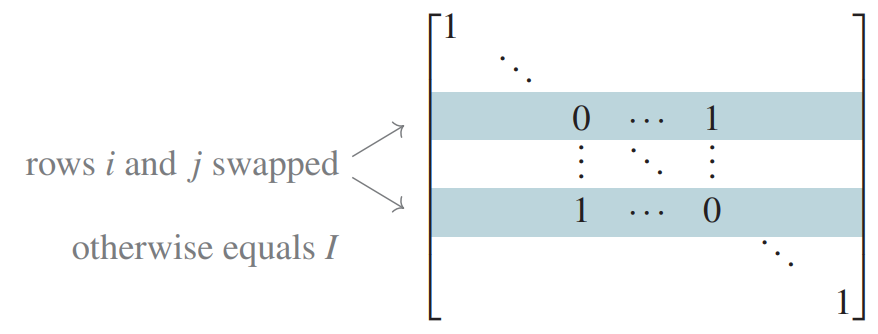
\includegraphics[height=0.28\textheight]{E1_swap.png}
    
    
% \end{figure}
% \pause

% Multiplying the $j$-th row of a matrix by a real number $c$ is the same as multiplying it by the following matrix on the left:
% \begin{figure}
%     \centering
%     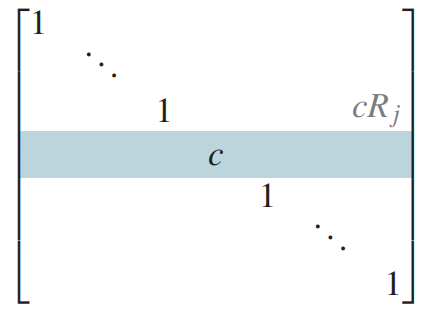
\includegraphics[height=0.28\textheight]{E2_mult.png}    
    
% \end{figure}



% \end{frame}


% \begin{frame}{Elementary Row Operations}
% Multiplying the $j$-th row of a matrix by a real number $c$ and adding it to the $i$-th row is the same as multiplying it by the following matrix on the left:
% \begin{figure}
%     \centering
%     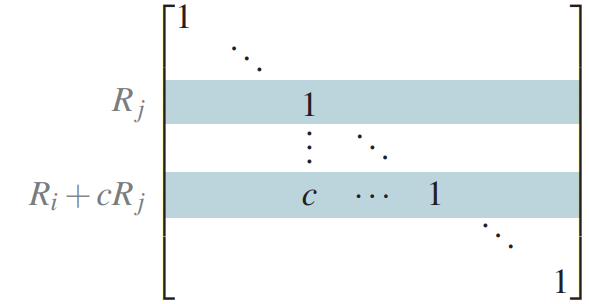
\includegraphics[height=0.28\textheight]{E3_add.png}    
    
% \end{figure}
% \pause Together, these matrices are called \textbf{elementary matrices}.


% \pause Since multiplying on the left by an elementary matrix is equivalent to
% performing a single elementary row operation, multiplying on the left by \textit{several}
% elementary matrices, one after another, must be equivalent to performing a
% \textit{sequence} of elementary row operations.

% \end{frame}





% % \begin{frame}{Gaussian Elimination}
% \begin{frame}{Row-Echelon Form}
%   \begin{block}{Definition}
% A matrix is in \textbf{row-echelon form} (REF) if it satisfies the following conditions:
%       \begin{enumerate}
%         \item[1.] All zero rows (consisting entirely of zeros) are at the bottom.
%         \item[2.] The first nonzero entry from the left in each nonzero row is a 1, called the \textbf{leading 1} for that row.
%         \item[3.] Each leading 1 is to the right of all leading 1s in the rows above it.

%       \end{enumerate}
%   % \end{block}
% \pause
% % \begin{block}{Definition}
%     A row-echelon matrix is said to be in \textbf{reduced row-echelon form} (RREF) if, in addition, it satisfies the following condition:
% \begin{enumerate}
%     \item[4.] Each leading 1 is the \textit{only} nonzero entry in its column.
% \end{enumerate}
% \end{block}

% \end{frame}



% \begin{frame}{Row-Echelon Form}

% The row-echelon matrices have a “staircase” form:

%   \begin{center}
%     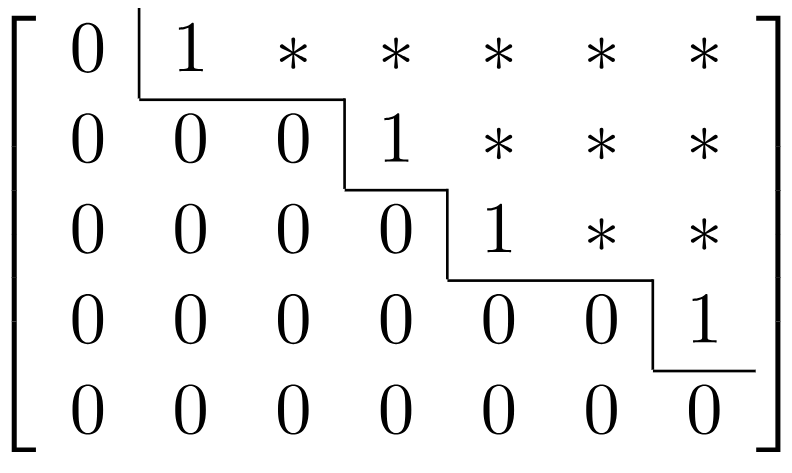
\includegraphics[width=0.6\textwidth, height=\textheight, keepaspectratio]{ref.png}
%   \end{center}
% \end{frame}

% % \begin{frame}{Gaussian Elimination}
% \begin{frame}{Row-Echelon Form}
  
%   \begin{example}
%     Matrices in Row-Echelon Form:
%     \[
%     \begin{bmatrix}
%       1 & 2 & 3 \\
%       0 & 1 & 4 \\
%       0 & 0 & 1
%     \end{bmatrix}, \qquad 
%     \begin{bmatrix}
%       1 & 6 & 3 \\
%       0 & 1 & 4 \\
%       0 & 0 & 1\\
%       0 & 0 & 0
%     \end{bmatrix}\]
%   \end{example}
  
%   \pause
  
%   \begin{example}
%     Matrices \textbf{not} in Row-Echelon Form:
%     \[
%     \begin{bmatrix}
%       1 & 2 & 3 \\
%       0 & 0 & 1 \\
%       0 & 1 & 4
%     \end{bmatrix}, \qquad 
%     \begin{bmatrix}
%       4 & 2 & 3 \\
%       0 & 1 & 1 \\
%       0 & 0 & 4
%     \end{bmatrix}, \qquad 
%     \begin{bmatrix}
%       1 & 2 & 3 \\
%       0 & 0 & 0 \\
%       0 & 0 & 1
%     \end{bmatrix}
%     \]
%   \end{example}
  
% \end{frame}

% \begin{frame}{Row-Echelon Form}
%     \begin{example}
%     Matrices in Reduced Row-Echelon Form:
%     \[
%     \begin{bmatrix}
%       1 & 0 & 0 \\
%       0 & 1 & 0 \\
%       0 & 0 & 1
%     \end{bmatrix}, \qquad 
%     \begin{bmatrix}
%       1 & 0 & 0 \\
%       0 & 1 & 0 \\
%       0 & 0 & 1\\
%       0 & 0 & 0
%     \end{bmatrix}, \qquad 
%     \begin{bmatrix}
%       1 & 0 & 0&0 \\
%       0 & 1 & 0 &0\\
%       0 & 0 & 0&0\\
%     \end{bmatrix}
%     \]
%   \end{example}

%   \pause \begin{block}{Remark}
%       Matrices of any shape can be transformed to Row-Echelon Form.
%   \end{block}\pause \begin{block}{Remark}
%       Matrices in Reduced Row-Echelon Form always contain a unit matrix $I$ in their upper left side.
%   \end{block}
  
% \end{frame}






% \begin{frame}{Row-Echelon Form}
%    If we could, applying elementary row operations, bring the augmented matrix $[\,A|\vb\,]$ to Row-Echelon Form, for example:
%   \[
%   [\,A|\vb\,] \equiv \begin{bmatrix}
%     1 & 3 & 2 & | & 10 \\
%     0 & 1 & 1 & | & 20 \\
%     0 & 0 & 1 & | & 30
%   \end{bmatrix}
%   \]
%   \pause That would mean:
%   \[ \begin{cases}
%       x+3y+2z=10\\
%       y+z=20\\
%       z=30
%   \end{cases}\]
%   which could be easily solved by substituting $z=30$, etc.\\
%   \pause How can we achieve that?
  
% \end{frame}


% \begin{frame}{Row-Echelon Form}
%    \begin{block}{Theorem}
%        Every matrix can be brought to (Reduced) Row-Echelon Form by a sequence of elementary row operations.
%    \end{block}\pause

%    \textbf{Gaussian Algorithm:}
%        \begin{description}[<+->]
%        \item[Step 1.] If the matrix consists entirely of zeros, \alert{stop}.
       
%        \item[Step 2.] Otherwise, find the row that contains the leftmost nonzero entry of the matrix (call that entry $a$).
       
%        \item[Step 3.] Move that row to the top position.
       
%        \item[Step 4.] Multiply that row by $\frac{1}{a}$ to create a leading 1.

%        \item[Step 5.] By subtracting multiples of that row from rows \textit{below it}, make the entries below the leading 1 in that column all 0.

%        \item[Step 6.] Fix the first row, and repeat steps 1–5 on the matrix consisting of the remaining rows
       
%        (\textit{we don't touch the first row anymore}).
%    \end{description}

% \end{frame}


% \begin{frame}{Row-Echelon Form}
%    \begin{example}
%        Solve the following system of equations:
%        \[ \begin{cases}
%            3x+y-4z&=-1\\
%            x+10z&=5\\
%            4x+y+3z&=1
%        \end{cases}\]
%        \pause The corresponding augmented matrix is\pause
% \[\begin{bmatrix}
%     3&1&-4&\vert&-1\\
%     1&0&10&\vert&5\\
%     4&1&3&\vert&1
% \end{bmatrix} \pause\xrightarrow{R_1\leftrightarrow R_2} \begin{bmatrix}
%     1&0&10&\vert&5\\
%     3&1&-4&\vert&-1\\
%     4&1&3&\vert&1
% \end{bmatrix}\]\[\pause \xrightarrow{R_2-3 R_1}\begin{bmatrix}
%     1&0&10&\vert&5\\
%     0&1&-34&\vert&-16\\
%     4&1&3&\vert&1
%     \end{bmatrix}
%     \pause\xrightarrow{R_3-4 R_1} \begin{bmatrix}
%     1&0&10&\vert&5\\
%     0&1&-34&\vert&-16\\
%     0&1&-37&\vert&1
% \end{bmatrix}
% \]

%    \end{example}
      

% \end{frame}
% \begin{frame}{Row-Echelon Form}
%    \begin{example}
   
%        \[ \xrightarrow{R_3- R_2} \begin{bmatrix}
%     1&0&10&\vert&5\\
%     0&1&-34&\vert&-16\\
%     0&0&-3&\vert&17
% \end{bmatrix}\pause\xrightarrow{-\frac{1}{3} R_3} \begin{bmatrix}
%     1&0&10&\vert&5\\
%     0&1&-34&\vert&-16\\
%     0&0&1&\vert&-\frac{17}{3}
% \end{bmatrix} \]\pause
% We have brought it to REF. This matrix means that the following reduced SLE:
% \[\begin{cases}
%     x+10z = 5\\
%     y-34z=-16\\
%     z=-\frac{17}{3}
% \end{cases} 
% \]
% is equivalent to the original system.\pause That is, the two have the same solutions:
% \[x=5-10z=-\frac{155}{3}, \qquad y=34z-16=-\frac{530}{3},\qquad z=-\frac{17}{3} \]

%    \end{example}
      

% \end{frame}


% \begin{frame}{Row-Echelon Form}
%   %   As we have seen, we can only 
%   % \begin{itemize}
%   %   \item In the context of Gaussian elimination:
%   %     \begin{enumerate}
%   %       \item If during the elimination process, a row of the form \([0 \, 0 \, \ldots \, 0 \, | \, a]\) is obtained where \(a\) is non-zero, the system is inconsistent.
%   %       \item The inconsistency arises because the system is trying to equate a non-zero value to zero, leading to a contradiction.
%   %     \end{enumerate}
%   % \end{itemize}
  
%   % \pause
  
%   \begin{example}
%     Consider the system:
%     \[
%     \begin{cases}
%       2x + y &= 5 \\
%       4x + 2y &= 8
%     \end{cases}
%     \]\pause
%     \[\begin{bmatrix}
%         2&1&\vert&5\\4&2&\vert&8
%     \end{bmatrix}\xrightarrow{\frac{1}{2} R_1} \begin{bmatrix}
%             1&0.5&\vert&2.5\\
%             4&2&\vert&8
% \end{bmatrix}\xrightarrow{R_2-4 R_1} \begin{bmatrix}
%             1&0.5&\vert&2.5\\
%             0&0&\vert&-2
% \end{bmatrix}\]\pause
% This corresponds to the equivalent system
% \[
%     \begin{cases}
%       x + 0.5y &= 2.5 \\
%       0x + 0y &= -2
%     \end{cases}
%     \]
% \pause
%     The second equation has no solution, so the system is inconsistent.
%   \end{example}\pause
%   As we have seen, if during the elimination process a row of the form \([0 \: 0 \: \ldots \: 0 \: | \: a]\) is obtained (where \(a\ne0\)), the system is inconsistent. 
% \end{frame}



% \begin{frame}{Row-Echelon Form}
%   What if after the elimination process we came up with the following system?
% \[
%     \begin{cases}
%       x + 0.5y &= 2.5 \\
%       0x + 0y &= 0
%     \end{cases}
%     \]
% \pause

%     For which values of $x$ and $y$ does this equality hold?
%     \[0x + 0y = 0 \]\pause For absolutely \textbf{any} $x$ and $y$! \pause

%     For example, $y$ can be any real number $a$, and $x$ will be $2.5-0.5a$, for any $a\in\R$. In this case we say that $y$ is a \textit{free variable} (because it can have any value).

    
% \end{frame}

% \begin{frame}{Gauss-Jordan Elimination}
\pause 

\begin{block}{Theorem (very fundamental)}
 The system $A\vx = \vb$ has a unique solution for any vector $\vb \in \mathbb{R}^n$, if and only if $\det A \ne 0$ (i.e. $A$ is invertible).
\end{block}
% \pause
% Using this important theorem, we are able to solve any SLE.
\end{frame}


% \begin{frame}{Gauss-Jordan Elimination}

% Gauss-Jordan elimination algorithm: 
%      \begin{description}[<+->]
%        \item[Step 1.] Carry the augmented matrix $[\,A\vert \vb\,]$ to a reduced row-echelon matrix using elementary row operations.
       
%        \item[Step 2.] If a row $ \left[ \begin{array}{ccccccc} 0 & 0 & 0 & \cdots & 0 &\vert& 1 \end{array} \right] $ occurs, the system is \textbf{inconsistent}.
       
%        \item[Step 3.] Otherwise, if there are any nonleading variables, assign them as parameters (treat them as arbitrary parameters $a, b, \dots$).
       
%        \item[Step 4.] Use the equations corresponding to the reduced row-echelon matrix to solve for the leading variables.
%    \end{description}
%    \pause If at the Step 3 we had no nonleading variables (hence no parameters) we will get a unique solution.
% \end{frame}




% \begin{frame}{Gauss-Jordan Elimination}
% \begin{example}
%     % Consider the system:
%     \[
%     \begin{cases}
        
%       x + 2y + z &= 4 \\
%       2x + 4y + 2z &= 8 \\
%       3x + 6y + 3z &= 12
%     \end{cases}
%     \]  \pause \\Let's write the augmented matrix $[\,A\vert \vb\,]$:    \begin{align*}
%      &\begin{bmatrix}
%         1 & 2 & 1 & | & 4 \\
%         2 & 4 & 2 & | & 8 \\
%         3 & 6 & 3 & | & 12
%       \end{bmatrix} \xrightarrow{R_2-2R_1} \begin{bmatrix}
%         1 & 2 & 1 & | & 4 \\
%         0 & 0 & 0 & | & 0 \\
%         3 & 6 & 3 & | & 12
%       \end{bmatrix} \xrightarrow{R_3-3R_1}  \begin{bmatrix}
%         1 & 2 & 1 & | & 4 \\
%         0 & 0 & 0 & | & 0 \\
%         0 & 0 & 0 & | & 0
%       \end{bmatrix} 
%     \end{align*}
%     We are left with $x+2y+z=4$. To solve that, we let $y=a, z=b$, and we get $x=4-2a-b$. Therefore, the solution is:
%     \[ x=4-2a-b,\qquad y=a,\qquad z=b,\qquad \text{for any }a,b\in\R\]
% \end{example}  

% \end{frame}


% \begin{frame}{Matrix Inverse}
% Yet another important application of Gauss-Jordan algorithm is finding the inverse of an invertible matrix.

% \begin{block}{Theorem}
%     If $A$ is an invertible matrix, there exists a sequence of elementary row operations that carry $A$ to the unit matrix $I$ of the same size. That same series of row operations carries $I$ to $A^{-1}$.
%   \begin{equation*} \left[ \begin{array}{ccc} A & \vert & I \end{array} \right] \rightarrow \left[ \begin{array}{ccc} I &\vert& A^{-1} \end{array} \right] \end{equation*}

% where the row operations on $A$ and $I$ are carried out simultaneously.
% \end{block}\pause
% What this means, is that to find the inverse of a $(n\times n)$ invertible matrix $A$ we need to write the augmented matrix $\left[ \begin{array}{ccc} A &\vert& I_n \end{array} \right]$ (of size $(n\times 2n)$) and perform Gauss-Jordan algorithm \textbf{to get $I$ on the left side}. What is left on the right side, is $A^{-1}$.

% \end{frame}




% \begin{frame}{Matrix Inverse}

% \begin{example}
%     Use the inversion algorithm to find the inverse of the matrix
%   \begin{equation*} A = \left[ \begin{array}{rrr} 2 & 7 & 1 \\ 1 & 4 & -1 \\ 1 & 3 & 0 \end{array} \right] \end{equation*}


%   \begin{equation*} \left[ \begin{array}{rrr} A &\vert& I \end{array} \right] = \left[ \begin{array}{rrr|rrr} 2 & 7 & 1 & 1 & 0 & 0 \\ 1 & 4 & -1 & 0 & 1 & 0 \\ 1 & 3 & 0 & 0 & 0 & 1 \end{array} \right] \end{equation*}

% First interchange rows 1 and 2.

%   \begin{equation*} \left[ \begin{array}{rrr|rrr} 1 & 4 & -1 & 0 & 1 & 0 \\ 2 & 7 & 1 & 1 & 0 & 0 \\ 1 & 3 & 0 & 0 & 0 & 1 \end{array} \right] \end{equation*}

% \end{example}
% \end{frame}






% \begin{frame}{Matrix Inverse}
% \begin{example}

% Next subtract 2 times row 1 from row 2, and subtract row 1 from row 3.
%   \begin{equation*} \left[ \begin{array}{rrr|rrr} 1 & 4 & -1 & 0 & 1 & 0 \\ 0 & -1 & 3 & 1 & -2 & 0 \\ 0 & -1 & 1 & 0 & -1 & 1 \end{array} \right] \end{equation*}
% Continue to reduced row-echelon form.
%   \begin{equation*} \left[ \begin{array}{rrr|rrr} 1 & 0 & 11 & 4 & -7 & 0 \\ 0 & 1 & -3 & -1 & 2 & 0 \\ 0 & 0 & -2 & -1 & 1 & 1 \end{array} \right] \quad\to\quad \left[ \def\arraystretch{1.5} \begin{array}{rrr|rrr} 1 & 0 & 0 & \frac{-3}{2} & \frac{-3}{2} & \frac{11}{2} \\ 0 & 1 & 0 & \frac{1}{2} & \frac{1}{2} & \frac{-3}{2} \\ 0 & 0 & 1 & \frac{1}{2} & \frac{-1}{2} & \frac{-1}{2} \end{array} \right] \end{equation*}

% Hence $A^{-1} = \dfrac{1}{2} \left[ \begin{array}{rrr} -3 & -3 & 11 \\ 1 & 1 & -3 \\ 1 & -1 & -1 \end{array} \right]$.
% \end{example}
% \end{frame}


% \begin{frame}{Matrix Inverse}
% \begin{example}
% Let's find the inverse of the following matrix:\[
% A = \begin{bmatrix}
% 2 & 2\\
% 4 & 5
% \end{bmatrix}
% \]\pause
% \begin{align*}
% \begin{bmatrix}
% 2 & 2 & \vert & 1 & 0 \\
% 4 & 5 & \vert & 0 & 1
% \end{bmatrix}&
% \underset{R_2-2R_1}{\longrightarrow}
% \begin{bmatrix}
% 2 & 2 & \vert & 1 & 0 \\
% 0 & 1 & \vert & -2 & 1
% \end{bmatrix} \\
% &\underset{R_1-2R_2}{\longrightarrow}
% \begin{bmatrix}
% 2 & 0 & \vert & 5 & -2 \\
% 0 & 1 & \vert & -2 & 1
% \end{bmatrix}
% \underset{\frac{1}{2}R_1}{\longrightarrow}
% \begin{bmatrix}
% 1 & 0 & \vert & \frac{5}{2} & -1 \\
% 0 & 1 & \vert & -2 & 1
% \end{bmatrix}
% \end{align*}\pause

% Therefore, $A^{-1} = \begin{bmatrix}
% \frac{5}{2} & -1 \\
%  -2 & 1
% \end{bmatrix}.$

% \end{example}
% \end{frame}


% % slide 2: Gauss Jordan det
% \begin{frame}{Determinant}
% Besides helping to bring a matrix to REF, elementary row operations also let us calculate the determinant much easier.\pause

% Before proceeding, let's state the following property:
% \begin{block}{Property}
%     If all entries of a matrix above or below its main diagonal are zeroes, then its determinant is equal to the product of the entries on its diagonal.
% \end{block}
% \pause
% \begin{example}
%     \begin{equation*}\left| \begin{array}{rrr} 3 & 8 & 13 \\ 0 & 4 & -13 \\ 0 & 0 & 1 \end{array} \right| = 3 \cdot 4 \cdot 1 = 12\end{equation*}
% \end{example}
%     % \begin{example}
        
%     %     $$A = \begin{bmatrix}
%     %         2 & 1 & -1 \\
%     %         1 & -3 & 2 \\
%     %         4 & 2 & 3 \\
%     %     \end{bmatrix}$$    
        
%     % \begin{equation*}
%     %            \begin{bmatrix}
%     %         2 & 1 & -1 \\
%     %         1 & -3 & 2 \\
%     %         4 & 2 & 3 \\
%     %     \end{bmatrix}
%     %      \xrightarrow{R_1\leftrightarrow R_2} 
%     %     \begin{bmatrix}
%     %         1 & -3 & 2 \\
%     %         2 & 1 & -1 \\
%     %         4 & 2 & 3 \\
%     %     \end{bmatrix}
%     %      \xrightarrow{R_2-2R_1} 
%     %     \begin{bmatrix}
%     %         1 & -3 & 2 \\
%     %         0 & 7 & -5 \\
%     %         4 & 2 & 3 \\
%     %     \end{bmatrix}
%     %      \xrightarrow{R_3-4 R_1} 
%     %     \end{equation*}
%     %     \begin{equation*}
%     %     \begin{bmatrix}
%     %         1 & -3 & 2 \\
%     %         0 & 7 & -5 \\
%     %         0 & 14 & -5 \\
%     %     \end{bmatrix}
%     %      \xrightarrow{R_3-2 R_2} 
%     %     \begin{bmatrix}
%     %         1 & -3 & 2 \\
%     %         0 & 7 & -5 \\
%     %         0 & 0 & 5 \\
%     %     \end{bmatrix}
%     %      \xrightarrow{\frac{1}{7}R_2, \: \frac{1}{5}R_3} 
%     %     \begin{bmatrix}
%     %         1 & -3 & 2 \\
%     %         0 & 1 & -\frac{5}{7} \\
%     %         0 & 0 & 1 \\
%     %     \end{bmatrix}\pause := B
%     % \end{equation*}
        
%     % \end{align*}
% % \end{example}

% \end{frame}


% % % slide 2: Gauss Jordan det
% % \begin{frame}{Determinant}
% % Besides helping to bring a matrix to REF, elementary row operations also let us calculate the determinant much easier. Consider the matrix $B$:
% % \[ B=\begin{bmatrix}
% %             1 & -3 & 2 \\
% %             0 & 1 & -\frac{5}{7} \\
% %             0 & 0 & 1 \\
% %         \end{bmatrix} \]
% % which was obtained by performing elementary row operations on
% % \[ A=\begin{bmatrix}
% %             2 & 1 & -1 \\
% %             1 & -3 & 2 \\
% %             4 & 2 & 3 \\
% %         \end{bmatrix}\] \pause
% % In this case, $A \sim B$. How are two row equivalent matrices related?
% % \end{frame}


% % slide 2: Gauss Jordan det
% \begin{frame}{Determinant}
% \begin{block}{Definition}
%     Two matrices $A$ and $B$ are called \textbf{row equivalent} (denoted by $A \sim B$) if it is possible to transform $A$ into $B$ by a sequence of elementary row operations.
% \end{block}
% \pause
% \begin{block}{Theorem}
%    % Let $A$ denote an $n \times n$ matrix.
% \begin{enumerate}[<+->]
%     \item If $B\sim A$ and $\det(B)=0$, then $\det(A)=0$.
%     \item If $A$ has a row/column of zeros, $\det(A)= 0$.
%     \item If two rows/columns of $A$ are identical, $\det(A) = 0$.
%     \item If two rows/columns of $A$ are swapped, the determinant \\becomes $-\det(A)$.
%     \item If a row/column of $A$ is multiplied by a constant $c$, the determinant becomes $c\cdot \det(A)$.
%     \item If a multiple of one row/column of $A$ is added to a different row/column, the determinant remains unchanged.
% \end{enumerate}

% \end{block}

% \end{frame}



% % slide 2: Gauss Jordan det
% \begin{frame}{Determinant}
% \begin{example}
%     \[A = \left[ \begin{array}{rrr} 1 & -1 & 3 \\ 1 & 0 & -1 \\ 2 & 1 & 6 \end{array} \right]\]\pause
%     \begin{equation*} \det(A) = \left| \begin{array}{rrr} 1 & -1 & 3 \\ 1 & 0 & -1 \\ 2 & 1 & 6 \end{array} \right| = \left| \begin{array}{rrr} 1 & -1 & 4 \\ 1 & 0 & 0 \\ 2 & 1 & 8 \end{array} \right| = - \left| \begin{array}{rr} -1 & 4 \\ 1 & 8 \end{array} \right| =12 \end{equation*}
% \end{example}
% \pause We added the first column to the third, then calculated the determinant by the cofactor method.
% \end{frame}


% % slide 2: Gauss Jordan det
% \begin{frame}{Determinant}
% % Elementary row operations are especially useful when calculating determinants of large matrices:
%    \begin{example}
        
%         $$A = \begin{bmatrix}
%             2 & 1 & -1 \\
%             1 & -3 & 2 \\
%             4 & 2 & 3 \\
%         \end{bmatrix}$$    
        
%     \begin{align*}
%            \det(A) = &\left| \begin{array}{rrr}   2 & 1 & -1 \\
%             1 & -3 & 2 \\
%             4 & 2 & 3 \end{array} \right| = -\left| \begin{array}{rrr}   1 & -3 & 2 \\
%             2 & 1 & -1 \\
%             4 & 2 & 3 \end{array} \right| = - \left| \begin{array}{rrr}  1 & -3 & 2 \\
%             0 & 7 & -5 \\
%             4 & 2 & 3 \end{array} \right| \\&= - \left| \begin{array}{rrr} 1 & -3 & 2 \\
%             0 & 7 & -5 \\
%             0 & 14 & -5 \end{array} \right| = - \left| \begin{array}{rrr}  1 & -3 & 2 \\
%             0 & 7 & -5 \\
%             0 & 0 & 5 \end{array} \right| =-35
%                 \end{align*}
% \end{example}
% \end{frame}













% Slide 0: linear comb

\begin{frame}{Linear Combination}

  \begin{block}{Definition}
    Given vectors \(\mathbf{v}_1, \mathbf{v}_2, \ldots, \mathbf{v}_k\) and scalars \(c_1, c_2, \ldots, c_k\), the expression
    \[ c_1\mathbf{v}_1 + c_2\mathbf{v}_2 + \ldots + c_k\mathbf{v}_k \]
    is called a \textbf{linear combination} of the vectors \(\mathbf{v}_1, \mathbf{v}_2, \ldots, \mathbf{v}_k\).
  \end{block}

  \pause

  \begin{example}
    Let \(\mathbf{v}_1 = \begin{bmatrix} 1 \\ 0 \end{bmatrix}\) and \(\mathbf{v}_2 = \begin{bmatrix} 0 \\ 1 \end{bmatrix}\). Then, the linear combination
    \[ 3\mathbf{v}_1 - 2\mathbf{v}_2 \]
    is equal to
    \[ 3\begin{bmatrix} 1 \\ 0 \end{bmatrix} - 2\begin{bmatrix} 0 \\ 1 \end{bmatrix} = \begin{bmatrix} 3 \\ -2 \end{bmatrix} \]
  \end{example}
\end{frame}

% \begin{frame}{Span}
%     \begin{block}{Definition}
%     The span of a set of vectors is the set of all possible linear combinations of those vectors:
%      \[
%     \text{span}\{\vv_1, \vv_2, \ldots, \vv_n\} = \{c_1\vv_1 + c_2\vv_2 + \ldots + c_n\vv_n \,|\, c_1, c_2, \ldots, c_n \in \mathbb{R}\}
%     \]
%   \end{block}
%   Given vectors $\{\vv_1, \vv_2, \ldots, \vv_n\}$, we also denote their span by $<\vv_1, \vv_2, \ldots, \vv_n>$.
  
%   \pause
%  \begin{block}{Property}
%      The span of a set of vectors is always a vector space.
%  \end{block}Geometrically, the span represents the subspace that can be formed by adding multiples of the given vectors.\pause  
%  \begin{block}{Definition}
%     If a vector space $V = \text{span}\{\vv_{1}, \dots, \vv_{n}\}$, we say that the vectors $\vv_{1}, \dots, \vv_{n}$ are spanning $V$.
%   \end{block}
 
% \end{frame}

% \begin{frame}{Span}

%       \begin{center}
%     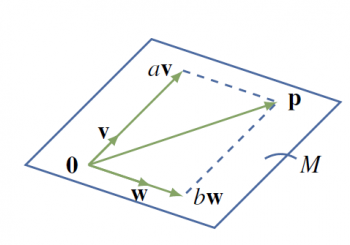
\includegraphics[width=0.6\textwidth, height=\textheight, keepaspectratio]{span.png}
%   \end{center}

%   In this example, the span of $\vv$ and $\vw$ contains any randomly selected vector $\mathbf{p}$. That means, $\vv$ and $\vw$ span $\R^2$.

%    \textcolor{blue}{Check these animations:\\ - \url{www.desmos.com/calculator/9rnbn0ycdd}\\ - \url{www.desmos.com/calculator/aje8cboe0j} }
% \end{frame}

% \begin{frame}{Span}

% \begin{example}
%     The span of \[
%     \vv_1 = \begin{bmatrix} 1 \\ 0\end{bmatrix} \quad \text{and} \quad \vv_2 = \begin{bmatrix} 0\\ 1 \end{bmatrix}
%     \]
%     \[<\vv_1,\vv_2>=\R^2.\]
% \end{example}\pause
%  \begin{example}
%     % Consider two vectors in $\mathbb{R}^2$:
%     \[
%     \vv_1 = \begin{bmatrix} 1 \\ 1 \end{bmatrix} \quad \text{and} \quad \vv_2 = \begin{bmatrix} 2 \\ 2 \end{bmatrix}
%     \]
%     \pause
%     % The span of $\{\vv_1, \vv_2\}$ is the set of all possible linear combinations of these vectors:
%     \[  <\{\vv_1, \vv_2\}> = \{c_1\vv_1 + c_2\vv_2 \,|\, c_1, c_2 \in \mathbb{R}\}= \{\begin{bmatrix} c_1+2c_2 \\ c_1+2c_2 \end{bmatrix} \,|\, c_1, c_2 \in \mathbb{R}\}
%     \]    \pause    This span forms the set of all $\begin{bmatrix}
%         a\\a
%     \end{bmatrix}$ vectors ($a\in\R$) in 2D.
%   \end{example}
% \end{frame}

% \begin{frame}{Linear Independence}
%     \begin{block}{Definition}
%          A set of vectors $\{\vv_1, \vv_2, \ldots\}$ is said to be \textbf{linearly independent} if no vector in the set can be written as a linear combination of the others \pause or, equivalently, if the equation
%     \[
%     c_1\vv_1 + c_2\vv_2 + \ldots + c_n\vv_n = \mathbf{0}
%     \]
%     can \textit{only} be true if $c_1 = c_2 = \ldots = c_n = 0$.

%     Otherwise, they are called \textbf{linearly dependent}.
%     \end{block}
    
%     \pause\begin{example}
%         $\va=\begin{bmatrix}
%             1\\0
%         \end{bmatrix}$ and $\vb=\begin{bmatrix}
%             0\\1
%         \end{bmatrix}$ are linearly independent.
%     \end{example}
% \end{frame}


% \begin{frame}{Linear Independence}

%       \begin{center}
%     \includegraphics[width=0.45\textwidth, height=\textheight, keepaspectratio]{ind.png}
%   \end{center}
% \end{frame}

% \begin{frame}{Linear Independence}
%     \begin{block}{Remark 1}
%         If at least one of the vectors $\vv_1,\dots,\vv_n$ is $\textbf{0}$, they are linearly dependent.
%     \end{block}

%     \begin{block}{Remark 2}
% The vectors $\vv_1,\dots,\vv_n$ are linearly dependent if and only if at least
% one of them is a linear combination of the others. \\In particular, if one
% vector is a multiple of another vector (i.e. $\vv_4=c\cdot \vv_2$) then the
% set $\{\vv_1,\dots,\vv_n\}$ is linearly dependent.
%     \end{block}
% For $n=2$, two vectors $\vv_1$ and $\vv_2$ are dependent if and only if one of them is a multiple (scaled version) of another: $\vv_1=k\cdot \vv_2$ or $\vv_2=k\cdot \vv_1$, i.e. if they lie on the same line.
 
% \end{frame}


% \begin{frame}{Basis}
% As we saw, vectors $\vv=\begin{bmatrix}
%     1\\0
% \end{bmatrix}$ and $\vw=\begin{bmatrix}
%     0\\1
% \end{bmatrix}$ are independent and span the 2D space. We also noticed visually that any 2D vector $\vu$ belongs to the span of $\vv$ and $\vw$\pause, or in other words, for any $\vu$, the vectors $\vv, \vu, \vw$ are linearly dependent.
% Vectors like these have a special name.

%     \begin{block}{Definition}
%         If $V$ is a vector space, a set $\{\vv_1,\vv_2,\dots,\vv_n\}$ of vectors in $V$ is called a \textbf{basis} of $V$ if it satisfies the following two conditions:
%         \begin{enumerate}
%             \item[1.] $\{\vv_1,\vv_2,\dots,\vv_n\}$ is linearly independent.
            
%             \item[2.] $\{\vv_1,\vv_2,\dots,\vv_n\}$ spans $V$, i.e. $V=<\vv_1,\vv_2,\dots,\vv_n>$
%         \end{enumerate}
%     \end{block}
% \pause \begin{block}{Property}
%     For any $n\in\N$, every set of $n$ linearly independent vectors form a basis of $\R^n$.
% \end{block}
% \end{frame}

% \begin{frame}{Basis}
%   \begin{example}
%     The vectors
%     $$\mathbf{e}_1 = \begin{bmatrix} 1 \\ 0 \end{bmatrix}, \quad \mathbf{e}_2 = \begin{bmatrix} 0 \\ 1 \end{bmatrix}
%     $$
%     form a basis for $\mathbb{R}^2$ and are called the \textbf{standard basis}. They are often denoted $\hat{i}, \hat{j}$.
%   \end{example}
  
%       \begin{center}
%     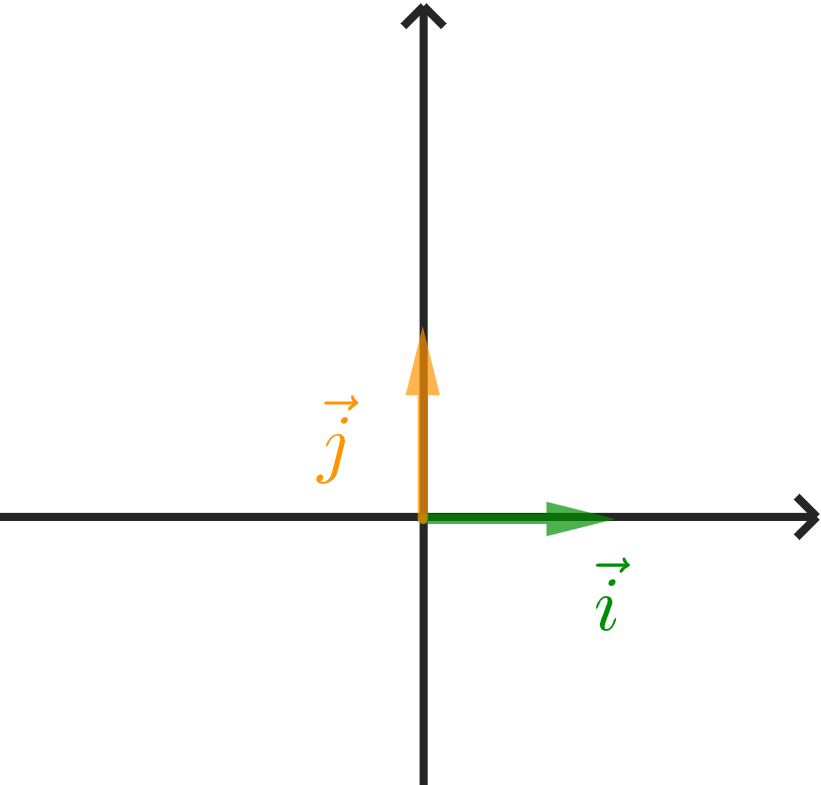
\includegraphics[width=0.5\textwidth, height=\textheight, keepaspectratio]{ij basis.png}
%   \end{center}
    
% \end{frame}

% \begin{frame}{Basis}
%   \begin{example}
%    The linearly independent vectors
%     \[
%     \vv_1 = \begin{bmatrix} 1 \\ 2 \end{bmatrix}, \quad \vv_2 = \begin{bmatrix} -1 \\ 1 \end{bmatrix}
%     \]
%     form a basis for $\mathbb{R}^2$
%     as these vectors are linearly independent and span the space.
%   \end{example}
  
%       \begin{center}
%     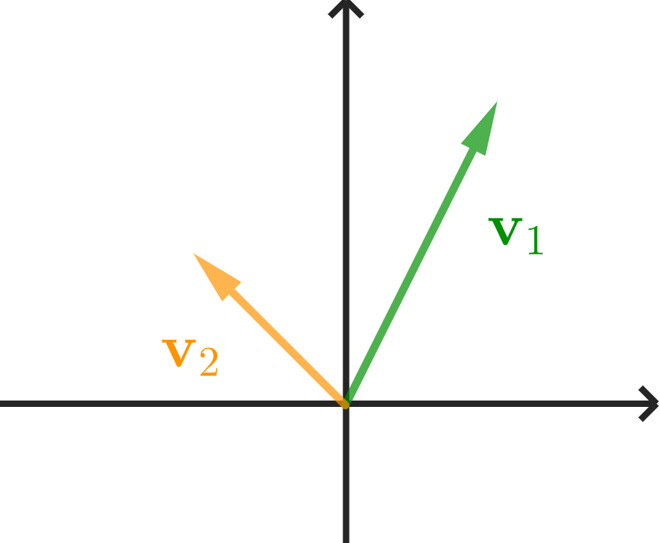
\includegraphics[width=0.5\textwidth, height=\textheight, keepaspectratio]{v1v2 basis.png}
%   \end{center}
    
% \end{frame}

% \begin{frame}{Basis}

%   \begin{example}
%     The vectors
%     \[
%     \mathbf{e}_1 = \begin{bmatrix} 1 \\ 0 \\ 0 \end{bmatrix}, \quad \mathbf{e}_2 = \begin{bmatrix} 0 \\ 1 \\ 0 \end{bmatrix}, \quad \mathbf{e}_3 = \begin{bmatrix} 0 \\ 0 \\ 1 \end{bmatrix}
%     \]
%     form a basis for $\mathbb{R}^3$ and are called the \textbf{standard basis}. They are often denoted $\hat{i}, \hat{j}, \hat{k}$.
%   \end{example}
%       \begin{center}
%     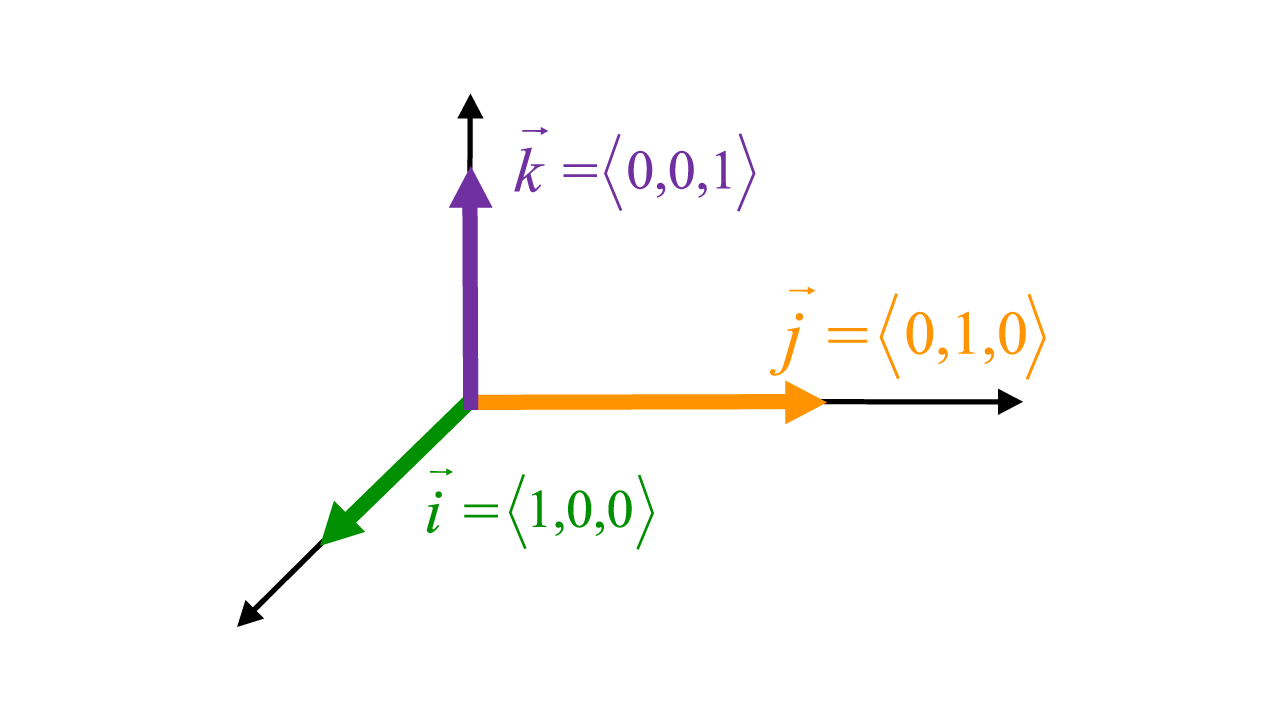
\includegraphics[width=0.5\textwidth, height=\textheight, keepaspectratio]{ijk.png}
%   \end{center}
    
% \end{frame}


% \begin{frame}{Basis}
% \begin{block}{Property}
%     Every vector space can have multiple bases, but all bases for a vector space have the same number of vectors.
% \end{block}\pause
% We call that number the \textbf{dimension} of the vector space.
%       \pause \begin{block}{Definition}
%     The number of vectors in any basis of the vector space $V$ is called the \textbf{dimension} of $V$, and is denoted $\text{dim}V$.
%   \end{block}
  
%   \pause
%   \begin{block}{Properties}
%   \begin{enumerate}
%       \item If $U$ is a subspace of $V$, $\text{dim}U\le\text{dim}V$.
%       \item Because $V=\{\textbf{0}\}$ is a vector space, it has a dimension. $\text{dim}V=0$.
%       \item $\text{dim}\R^n =n$.
%   \end{enumerate}
     
%   \end{block}
  
% \end{frame}


\begin{frame}{Span}
  Suppose we have some vectors $\vv_1, \vv_2,\dots,\vv_n\in V$ where $V$ is a vector space. Recall that any other vector that can be expressed as:
  \[c_1 \vv_1 + c_2 \vv_2 + \dots + c_n\vv_n\]
  is called a linear combination of $\vv_1,\dots,\vv_n$. \pause

  Let's call the set of \textit{all possible linear combinations} of $\vv_1,\dots,\vv_n$ their \textbf{span} and denote it by $\Span\{\vv_1,\dots,\vv_n\}$ or $<\vv_1, \ldots, \vv_n>$. \pause

 \begin{block}{Definition}
    The \textbf{span} of a set of vectors is the set of all possible linear combinations of those vectors:
     \begin{align*}
          \text{span}\{\vv_1, &\vv_2, \ldots, \vv_n\} = <\vv_1, \ldots, \vv_n> \\&=    \{c_1\vv_1 + c_2\vv_2 + \ldots + c_n\vv_n \,\mid\, c_1, c_2, \ldots, c_n \in \mathbb{R}\}
     \end{align*}
  \end{block}
  
 
\end{frame}


\begin{frame}{Span}
Geometrically, the span represents all the vectors that we can get by adding multiples of the given vectors.\pause  
      \begin{center}
    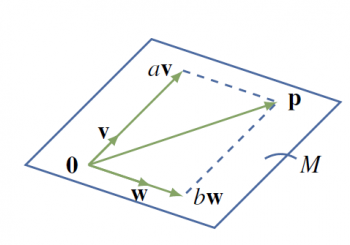
\includegraphics[width=0.6\textwidth, height=\textheight, keepaspectratio]{span.png}
  \end{center}

  For example, the span of $\vv$ and $\vw$ here contains any randomly selected vector $\mathbf{p}$. That means, $<\vv,\vw>=$\pause$\R^2$.

\end{frame}


\begin{frame}{Span}


 \begin{block}{Definition}
    If a vector space $V = \text{span}\{\vv_{1}, \dots, \vv_{n}\}$, we say that the vectors $\vv_{1}, \dots, \vv_{n}$ \textit{span} the space $V$.
  \end{block}

\pause In previous example, $\vv$ and $\vw$ span $\R^2$.
\pause \\ \\ \medskip A vector space can be spanned by a set of vectors, but is the span itself a vector space? \pause
  
 \begin{block}{Theorem}
     The span of a set of vectors \textbf{is always a vector space}.
 \end{block}

 
\end{frame}


\begin{frame}{Span}

\begin{example}
    The span of \(
    \vv_1 = \begin{bmatrix} 1 \\ 0\end{bmatrix} \; \text{and} \; \vv_2 = \begin{bmatrix} 0\\ 1 \end{bmatrix}
    \) is \pause    $<\vv_1,\vv_2>=\R^2.$
\end{example}\pause
 \begin{example}
     The span of \(
    \vv_1 = \begin{bmatrix} 1 \\ 1\end{bmatrix} \; \text{and} \; \vv_2 = \begin{bmatrix} 2\\ 2 \end{bmatrix}
    \) is
    \pause
    % The span of $\{\vv_1, \vv_2\}$ is the set of all possible linear combinations of these vectors:
    \[  <\vv_1, \vv_2> = \{c_1\vv_1 + c_2\vv_2 \,\mid\, c_1, c_2 \in \mathbb{R}\}= \left\{\begin{bmatrix} c_1+2c_2 \\ c_1+2c_2 \end{bmatrix} \,\mid\, c_1, c_2 \in \mathbb{R}\right\}
    \]    \pause   \[ = \left\{\begin{bmatrix} a \\ a \end{bmatrix} \,\mid\, a \in \mathbb{R}\right\} \subsetneq \R^2. \]\pause This span forms the set of vectors on the line $y=x$.
  \end{example}
\end{frame}

\begin{frame}{Linear Independence}

Why did the vectors of the first example span $\R^2$, while those in the second example didn't? \pause Because in the second example $\vv_2=2\vv_1$! \pause

    \begin{block}{Definition}
         A set of vectors $\{\vv_1, \vv_2, \ldots\}$ is said to be \textbf{linearly independent} if no vector in the set can be written as a linear combination of the others \pause or, equivalently, if the equation
    \[
    c_1\vv_1 + c_2\vv_2 + \ldots + c_n\vv_n = \mathbf{0}
    \]
    is \textit{only} true if $c_1 = c_2 = \ldots = c_n = 0$.

\pause
    Otherwise, the vectors are called \textbf{linearly dependent}.
    \end{block}
    
    \pause\begin{example}
        $\va=\begin{bmatrix}
            1\\0
        \end{bmatrix}$ and $\vb=\begin{bmatrix}
            0\\1
        \end{bmatrix}$ are linearly independent.
    \end{example}
\end{frame}


\begin{frame}{Linear Independence}

      \begin{center}
    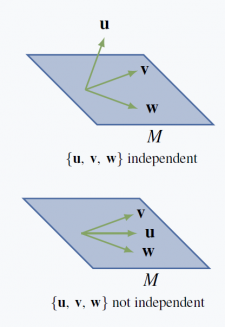
\includegraphics[width=0.35\textwidth, keepaspectratio]{lin-indep.png}
  \end{center}
  
       \textcolor{blue}{Check these animations:\\ - \url{www.desmos.com/calculator/9rnbn0ycdd}\\ - \url{www.desmos.com/calculator/aje8cboe0j} }
\end{frame}

\begin{frame}{Linear Independence}
    \begin{block}{Remark 1}
        If at least one of the vectors $\vv_1,\dots,\vv_n$ is $\textbf{0}$, they are linearly dependent.
    \end{block}
\pause
    \begin{block}{Remark 2}
The vectors $\vv_1,\dots,\vv_n$ are linearly dependent if and only if at least
one of them is a linear combination of the others.
    \end{block}
\pause
    \begin{block}{Remark 3}
        In particular, if one
vector is a multiple of another vector (e.g. $\vv_4=c\cdot \vv_2$) then the
set $\{\vv_1,\dots,\vv_n\}$ is linearly dependent.
    \end{block}
\pause
For $n=2$, two vectors $\vv_1$ and $\vv_2$ are dependent if and only if they lay on the same line, i.e. one of them is a multiple (scaled version) of another: $\vv_1=k\cdot \vv_2$ or $\vv_2=k\cdot \vv_1$. 
\pause \\

For $n=3$, three vectors $\vv_1, \vv_2$ and $\vv_3$ are dependent if and only if they lay in the same plane.

\end{frame}


\begin{frame}{Basis}
As we saw, vectors $\vv=\begin{bmatrix}
    1\\0
\end{bmatrix}$ and $\vw=\begin{bmatrix}
    0\\1
\end{bmatrix}$ are independent and span the 2D space. We also noticed visually that any 2D vector $\vu$ belongs to the span of $\vv$ and $\vw$\pause, or in other words, for any $\vu$, the vectors $\vv, \vu, \vw$ are linearly dependent. \pause

Vector sets like these have a special name.

    \begin{block}{Definition}
        If $V$ is a vector space, a set $\{\vv_1,\vv_2,\dots,\vv_n\}$ of vectors in $V$ is called a \textbf{basis} of $V$ if it satisfies the following two conditions:
        \begin{enumerate}
            \item[1.] $\{\vv_1,\vv_2,\dots,\vv_n\}$ is linearly independent.
            
            \item[2.] $\{\vv_1,\vv_2,\dots,\vv_n\}$ spans $V$, i.e. $V=<\vv_1,\vv_2,\dots,\vv_n>$
        \end{enumerate}
    \end{block}

\pause 

Equivalently, $\{\vv_1,\vv_2,\dots,\vv_n\}$ forms a basis of $V$ if for any $\vu \in V$ there exist \textbf{unique} numbers $c_1,c_2,\dots,c_n$ such that
\[\vu = c_1\vv_1+c_2\vv_2+\dots+c_n\vv_n.\]

\end{frame}

\begin{frame}{Basis}
  \begin{example}
    The vectors
    $$\mathbf{e}_1 = \begin{bmatrix} 1 \\ 0 \end{bmatrix}, \quad \mathbf{e}_2 = \begin{bmatrix} 0 \\ 1 \end{bmatrix}
    $$
    form a basis for $\mathbb{R}^2$ and are called the \textbf{standard basis}. They are often denoted $\hat{i}, \hat{j}$.
  \end{example}
  
      \begin{center}
    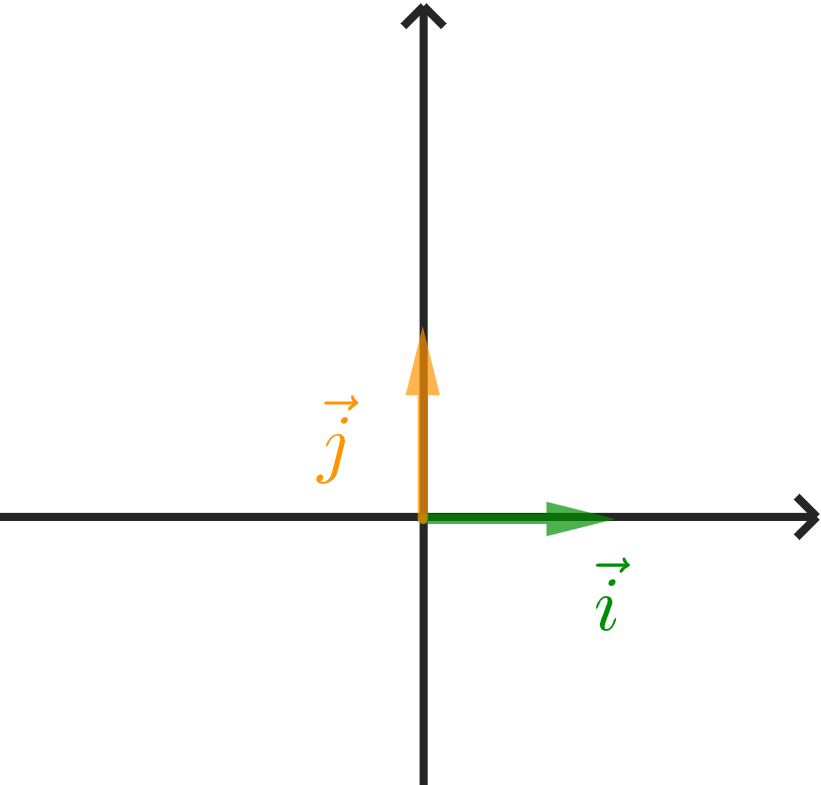
\includegraphics[width=0.3\textwidth, keepaspectratio]{ij basis.png}
  \end{center}
    
\end{frame}

\begin{frame}{Basis}
  \begin{example}
   The linearly independent vectors
    \[
    \vv_1 = \begin{bmatrix} 1 \\ 2 \end{bmatrix}, \quad \vv_2 = \begin{bmatrix} -1 \\ 1 \end{bmatrix}
    \]
    form a basis for $\mathbb{R}^2$
    as these vectors are linearly independent and span the space.
  \end{example}
  
      \begin{center}
    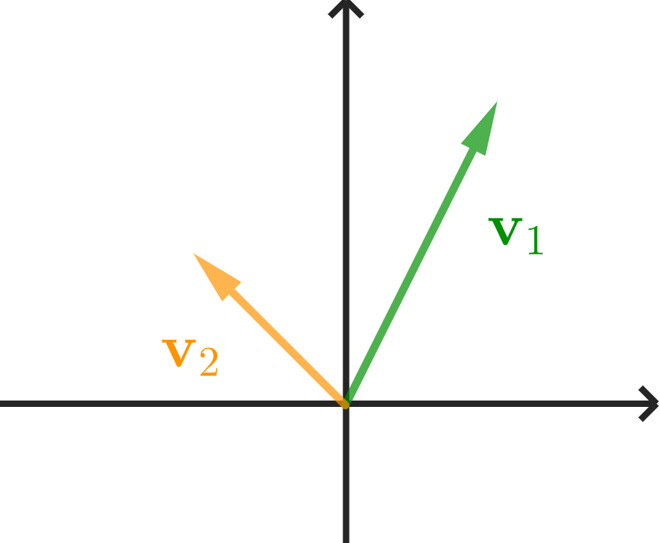
\includegraphics[width=0.3\textwidth,  keepaspectratio]{v1v2 basis.png}
  \end{center}
  
    
\end{frame}

\begin{frame}{Basis}

  \begin{example}
    The vectors
    \[
    \mathbf{e}_1 = \begin{bmatrix} 1 \\ 0 \\ 0 \end{bmatrix}, \quad \mathbf{e}_2 = \begin{bmatrix} 0 \\ 1 \\ 0 \end{bmatrix}, \quad \mathbf{e}_3 = \begin{bmatrix} 0 \\ 0 \\ 1 \end{bmatrix}
    \]
    form a basis for $\mathbb{R}^3$ and are called the \textbf{standard basis}. They are often denoted $\hat{i}, \hat{j}, \hat{k}$.
  \end{example}
      \begin{center}
    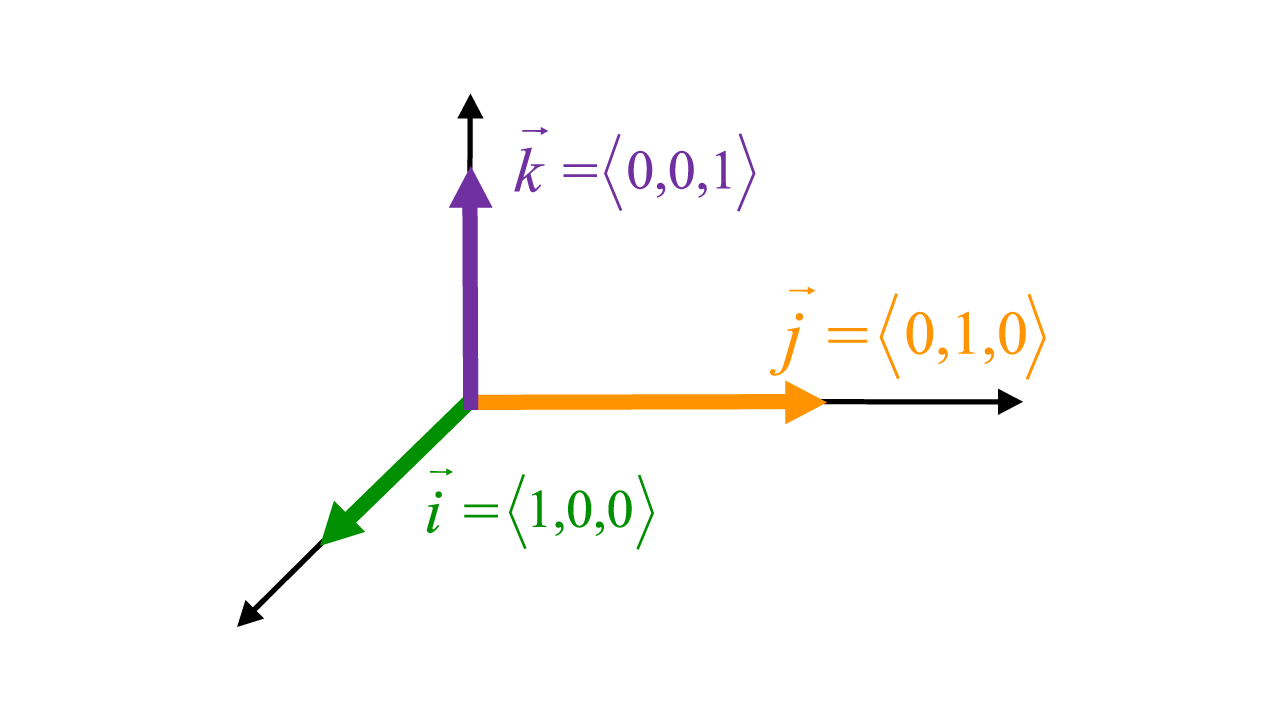
\includegraphics[width=0.5\textwidth, height=\textheight, keepaspectratio]{ijk.png}
  \end{center}
    
\end{frame}


\begin{frame}{Basis}

  \begin{example}
    The vectors
    \[
    \vv_1 = \begin{bmatrix} 0 \\ 1 \end{bmatrix}, \quad 
    \vv_2 = \begin{bmatrix} 1 \\ 1 \end{bmatrix} \quad 
    \vv_3 = \begin{bmatrix} 1 \\ 0 \end{bmatrix}
    \]
    \pause are not a basis for $\R^2$ because they are linearly dependent.
  \end{example}
  \pause
  
  \begin{example}
    The vectors
    \[
    \vv_1 = \begin{bmatrix} 1 \\ 0 \\ 0 \end{bmatrix}, \quad 
    \vv_2 = \begin{bmatrix} 0 \\ 1 \\ 0 \end{bmatrix} 
    \]
    \pause are not a basis for $\R^3$ because they don't span it.
  \end{example}
  
\end{frame}


\begin{frame}{Basis}
  
  \begin{example}
    The vectors
    \[
    \vv_1 = \begin{bmatrix} 1 \\ 0 \end{bmatrix}, \quad 
    \vv_2 = \begin{bmatrix} 4 \\ 0 \end{bmatrix} 
    \]
    \pause are not a basis for $\R^2$ because they neither span it, nor are linearly independent.
  \end{example}
  \pause
  
\begin{block}{Property}
    For any $n\in\N$, every set of $n$ linearly independent vectors form a basis of $\R^n$.
    \end{block}
\end{frame}

    
\begin{frame}{Basis}
As we have seen, there are more than one bases of $\R^2$, however all of them consist of two vectors. The same is true for any vector space.\pause

\begin{block}{Property}
    Any two bases of any vector space have the same number of vectors.
\end{block}\pause
      \begin{block}{Definition}
    The number of vectors in any basis of a vector space $V$ is called the \textbf{dimension} of $V$ and is denoted by $\text{dim}V$.
  \end{block}

  The dimension describes the "size" of a vector space. It shows how many linearly independent vectors are there in that vector space at most.
  \pause
  \begin{block}{Properties}
  \begin{enumerate}[<+->]
      \item If $U$ is a subspace of $V$, $\text{dim}U\le\text{dim}V$.
      \item Because $V=\{\textbf{0}\}$ is a vector space, it has a dimension. $\text{dim}V=0$.
      \item $\text{dim}\R^n =n$.
  \end{enumerate}
     
  \end{block}


  
\end{frame}

    



% slide 3: rank
\begin{frame}{Rank}

Time to get back to our matrices. Consider the following matrix:
        
        $$A = \begin{bmatrix}
            2 & 1 & -1 \\
            1 & -3 & 2 \\
            4 & 2 & 3 \\
        \end{bmatrix}$$    
        \pause
    \begin{equation*}
               \begin{bmatrix}
            2 & 1 & -1 \\
            1 & -3 & 2 \\
            4 & 2 & 3 \\
        \end{bmatrix}\pause
         \xrightarrow{R_1\leftrightarrow R_2} 
        \begin{bmatrix}
            1 & -3 & 2 \\
            2 & 1 & -1 \\
            4 & 2 & 3 \\
        \end{bmatrix}\pause
         \xrightarrow{R_2-2R_1} 
        \begin{bmatrix}
            1 & -3 & 2 \\
            0 & 7 & -5 \\
            4 & 2 & 3 \\
        \end{bmatrix}\pause
         \xrightarrow{R_3-4 R_1} 
        \end{equation*}
        \begin{equation*}
        \begin{bmatrix}
            1 & -3 & 2 \\
            0 & 7 & -5 \\
            0 & 14 & -5 \\
        \end{bmatrix}\pause
         \xrightarrow{R_3-2 R_2} 
        \begin{bmatrix}
            1 & -3 & 2 \\
            0 & 7 & -5 \\
            0 & 0 & 5 \\
        \end{bmatrix}\pause
         \xrightarrow{\frac{1}{7}R_2, \: \frac{1}{5}R_3} 
        \begin{bmatrix}
            1 & -3 & 2 \\
            0 & 1 & -\frac{5}{7} \\
            0 & 0 & 1 \\
        \end{bmatrix}\pause := B
    \end{equation*}


\pause So the REF of $A$ is $B$. There are 3 rows and each of them starts with a leading 1.
    
\end{frame}

\begin{frame}{Rank}
 This other matrix, for example, 
\[ C=\begin{bmatrix}
            3 & 2 & -5 \\
            -6 & -4 & 10 \\
            3 & 0 & 1 \\
        \end{bmatrix} \pause 
        \xrightarrow{R_2+2 R_1} 
        \begin{bmatrix}
        3 & 2 & -5 \\
            0 & 0 & 0 \\
            3 & 0 & 1 \\
         \end{bmatrix}
        \xrightarrow{R_2\leftrightarrow R_3} 
        \begin{bmatrix}
        3 & 2 & -5 \\
            3 & 0 & 1 \\
            0 & 0 & 0 \\
         \end{bmatrix}
        \xrightarrow{R_2- R_1} \]\[
        \begin{bmatrix}
        3 & 2 & -5 \\
            0 & -2 & 6 \\
            0 & 0 & 0 \\
         \end{bmatrix}
        \xrightarrow{-\frac{1}{2}R_2} 
        \begin{bmatrix}
        3 & 2 & -5 \\
            0 & 1 & -3 \\
            0 & 0 & 0 \\
         \end{bmatrix}
        \xrightarrow{\frac{1}{3}R_1} 
        \begin{bmatrix}
        1 & \frac{2}{3} & -\frac{5}{3} \\
            0 & 1 & -3 \\
            0 & 0 & 0 \\
         \end{bmatrix}:=D
        \]
\pause when brought to REF, has only two leading 1s. \pause 

\\ \\ \medskip What does it show?

\end{frame}




% slide 3: rank
\begin{frame}{Rank}
\begin{block}{Definition}
Let $A\in\R^{m\times n}$ be any matrix. The number of leading 1s in any Row Echelon Form of $A$ is called the \textbf{rank} of matrix $A$, and is denoted by $\rank(A)$.
\end{block}
\pause
\begin{example}
    \[ A \sim B=\begin{bmatrix}
            1 & -3 & 2 \\
            0 & 1 & -\frac{5}{7} \\
            0 & 0 & 1 \\
        \end{bmatrix} \quad \Rightarrow \quad \rank(A)=\rank(B)=3\]
    \[ C \sim D=\begin{bmatrix}
        1 & \frac{2}{3} & -\frac{5}{3} \\
            0 & 1 & -3 \\
            0 & 0 & 0 \\
         \end{bmatrix}  \quad \Rightarrow \quad \rank(C)=\rank(D)=2\]
\end{example}

\pause 

In other words, \textit{rank = number of non-zero lines in row-echelon form}.

\end{frame}



% slide 3: rank
\begin{frame}{Rank}
\begin{example}
 \[ A = \left[ \begin{array}{rrrr} 1 & 1 & -1 & 4 \\ 2 & 1 & 3 & 0 \\ 0 & 1 & -5 & 8 \end{array} \right]\]
  To calculate its rank, we should carry it to REF:
  \begin{equation*} A = \left[ \begin{array}{rrrr} 1 & 1 & -1 & 4 \\ 2 & 1 & 3 & 0 \\ 0 & 1 & -5 & 8 \end{array} \right] \rightarrow \left[ \begin{array}{rrrr} 1 & 1 & -1 & 4 \\ 0 & -1 & 5 & -8 \\ 0 & 1 & -5 & 8 \end{array} \right] \rightarrow \left[ \begin{array}{rrrr} 1 & 1 & -1 & 4 \\ 0 & 1 & -5 & 8 \\ 0 & 0 & 0 & 0 \end{array} \right] \end{equation*}

  It has two leading 1s, therefore $\rank(A) = 2$.
\end{example}

  
\end{frame}

% slide 3: rank
\begin{frame}{Rank}


\begin{block}{Definition}
    For any matrix $A$, the span of its columns is called the \textbf{column space} of $A$, and is denoted by $\text{colsp}(A)$.
\end{block}
\pause
\begin{block}{Definition}
    For any matrix $A$, the span of its rows is called the \textbf{row space} of $A$, and is denoted by $\text{rowsp}(A)$.
\end{block}
\pause
\begin{block}{Theorem}
For any matrix $A$, \[\rank(A) = \dim(\text{colsp}(A)) = \dim(\text{rowsp}(A)).\]
    % If $A\in\R^{m\times n}$ is a matrix with rows $A_1, A_2, \dots, A_m$ (each of length $n$), then $$\rank(A) = \dim(<A_1, A_2, \dots, A_n>).$$Equivalently, $\rank(A) = \dim(<{^1}A, {^2A}, \dots, {^nA}>)$, where ${^1A},\dots,{^nA}$ are the columns of $A$.
\end{block}
In other words, the rank of the matrix shows \textbf{how many of its rows/columns are linearly independent}, and this number turns out to be the same for both rows and columns.
\end{frame}


% slide 3: rank
\begin{frame}{Rank}
\begin{block}{Properties}
\begin{enumerate}[<+->]
    \item For any $A$, $\rank(A)=\rank(A^T)$,
    \item For any $A\in\R^{m\times n}$, $\rank(A) \le \min(m, n)$,
    \item For any square matrix $A\in\R^{n\times n}$, $A$ is invertible if and only if $\rank(A)=n$.\end{enumerate}
\end{block}
    \pause

Most importantly, if we take some vectors $\{\vv_1, \vv_2, \dots, \vv_n\}$ and write them as rows or columns of a matrix, the dimension of their span will equal the rank of that matrix. \\ 
\pause This important property helps us to find the number of solutions of SLEs:
\begin{block}{Theorem}
    If a system of $m$ equations in $n$ variables is consistent, and the rank of the \textit{augmented matrix} is $r$, then:
\begin{enumerate}
    \item[1. ] If $r < n$, the system has infinitely many solutions.
\item[2. ] If $r = n$, the system has a unique solution.
\end{enumerate}
\end{block}

\end{frame}


% slide 6: definite
\begin{frame}{Geometric Interpretation of Matrices}

Finally, what do matrices mean geometrically? \pause Think about them this way: when you multiply a, say, $2\times 2$ matrix $A$ by a vector $\vv\in\R^2$, what you get is another vector $\vu=A\vv\in\R^2$. We call this $\vu$ the \textbf{transformed version} of $\vv$ (and the matrix $A$ is called a linear transformation).
\pause

\begin{figure}
    \centering
    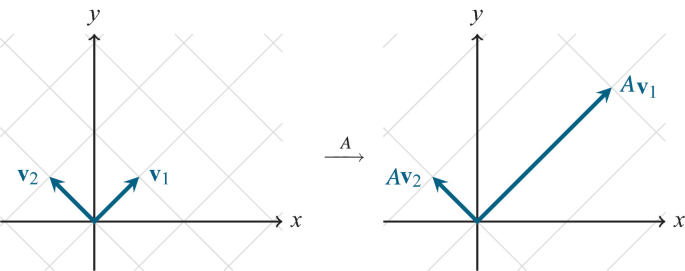
\includegraphics[width=0.75\linewidth]{viz ex.png}
    
    
\end{figure}

\end{frame}


% slide 6: definite
\begin{frame}{Geometric Interpretation of Matrices}

For example, the matrix $A = \begin{bmatrix}
    2&1\\1&2
\end{bmatrix}$ can be visualized this way:

\begin{figure}
    \centering
    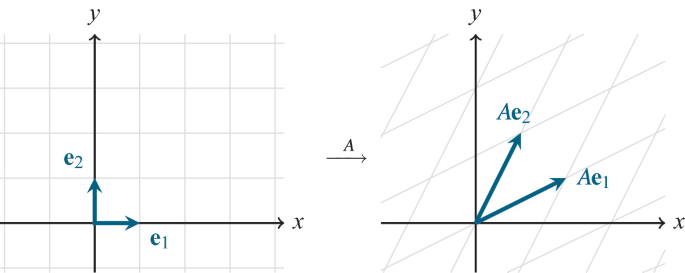
\includegraphics[width=0.75\linewidth]{viz Av.png}
    
    
\end{figure}

As we see, multiplication with a matrix \textbf{transforms the basis vectors} $\ve_1$ and $\ve_2$ into the \textbf{columns of the matrix}, $\begin{bmatrix}
    2\\1
\end{bmatrix}$ and $\begin{bmatrix}
    1\\2
\end{bmatrix}$, therefore any vector with coordinates $\begin{bmatrix}
    a\\b
\end{bmatrix}$ is transformed into $a\begin{bmatrix}
    2\\1
\end{bmatrix}+b\begin{bmatrix}
    1\\2
\end{bmatrix}$.
\end{frame}


\begin{frame}{Geometric Interpretation of Matrices}

When multiplying by the identity matrix $I=\begin{bmatrix}
    1&0\\0&1
\end{bmatrix}$, the vectors remain the same, i.e. $I$ does not change the vectors.  When multiplying by $\begin{bmatrix}
    1&0\\0&2
\end{bmatrix}$, the $y$-coordinate of all vectors doubles, i.e. this matrix stretches vectors along the $y$-axis by $2$ times.

\pause 

\bigskip

Some matrices are just rotating vectors by some degree or flipping them. Others scale them, or perform more complex transformations.   

\bigskip

\textcolor{blue}{Check different matrices yourself:\\ - \url{visualize-it.github.io/linear_transformations/simulation.html} 
\\ - \url{www.shad.io/MatVis}
}


    
\end{frame}


% slide 6: definite
\begin{frame}{Geometric Interpretation of Matrices}

And what about the determinant? If we look closely at the $1\times 1$ square formed by the basis vectors $\ve_1$ and $\ve_2$, we can see that their transformed versions, $A\ve_1$ and $A\ve_2$, form a parallelogram:

\begin{figure}
    \centering
    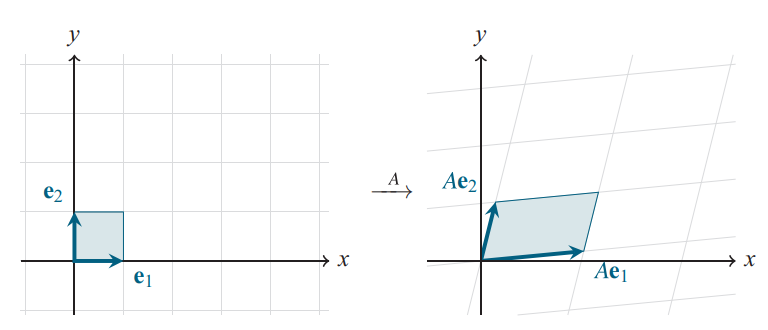
\includegraphics[width=0.75\linewidth]{viz det.png}
    
    
\end{figure}

\pause The area of that parallelogram is $\det(A)$.
\end{frame}



% slide 6: definite
\begin{frame}{Geometric Interpretation of Matrices}

In fact, after we apply the transformation $A$ (i.e. multiply every vector in $\R^2$ by $A$), the area of \textit{any shape} gets scaled by the factor of $\det(A)$:

\begin{figure}
    \centering
    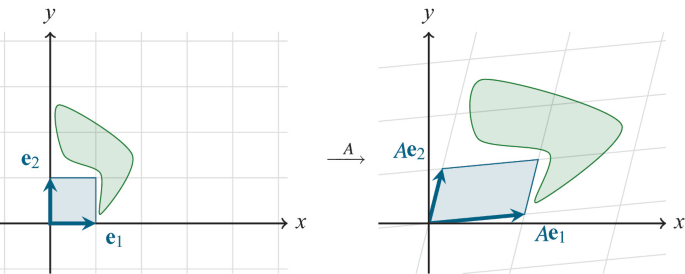
\includegraphics[width=0.75\linewidth]{viz area.png}
    
    
\end{figure}
% \pause

% Which is truly amazing.
\end{frame}


% % slide 4: geometric
% \begin{frame}{Geometric interpretation}
% Let's now move on to how we can visualize the matrices in 2D/3D spaces.

% %  [a,b,c] -> a*e1 + b*e2 + c*e3
% % isk vren vor A es kirarum -> ...
% % gcagri vra x
% % gcagri vra Ax
% % aysinqn es A-n nuynn a, vor ases` verj, bazisi vectornery poxvecin sranic heto sranq en
% % mi qani orinakner (shear rotation ban)
% % ranky vor < n => squish a anum
% % hima vorosh vectorneri uxxutyuny poxvum a (ex)
% % voroshneri miayn mecutyuny (ex)
% % dranc vonc anvanenq ?

% \end{frame}




% slide 6: definite
\begin{frame}{Geometric Interpretation of Matrices}

Sometimes the matrix also has some vectors which \textbf{do not change their direction} when being multiplied (transformed) by that matrix, rather they get scaled by some number:

\begin{figure}
    \centering
    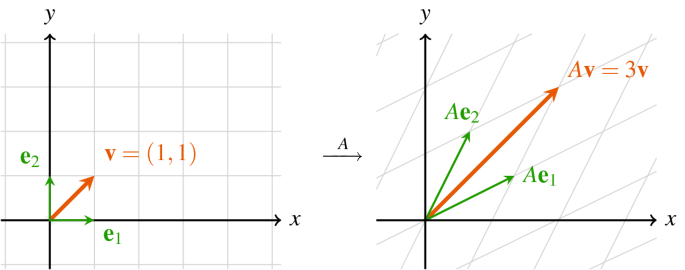
\includegraphics[width=0.75\linewidth]{viz eig.png}
    
\end{figure}

\pause

Vectors like these are of special interest to us, and we call them \textit{eigenvectors}.
\end{frame}




% slide 5: eigen
\begin{frame}{Eigenvalues and Eigenvectors}
\begin{block}{Definition}
    If $A$ is an $n \times n$ matrix, a number $\lambda$ is called an \textbf{eigenvalue} of $A$ if for some vector $\vv\ne\mathbf{0}$:
    \begin{equation*} A\vv = \lambda \vv\end{equation*}

In that case, $\vv$ is called an \textbf{eigenvector} of $A$ \textit{corresponding to} the eigenvalue $\lambda$.
\end{block}
\pause
\begin{example}
    For the matrix $A = \left[ \begin{array}{rr} 3 & 5 \\ 1 & -1 \end{array}\right]$ and vector $\vv = \left[ \begin{array}{r} 5 \\ 1 \end{array}\right]$,
    \[A\vv =  \left[ \begin{array}{rr} 3 & 5 \\ 1 & -1 \end{array}\right]\left[ \begin{array}{r} 5 \\ 1 \end{array}\right] = \left[ \begin{array}{r} 20 \\ 4 \end{array}\right] =4\vv\]
    so $\lambda = 4$ is an eigenvalue of $A$ with corresponding eigenvector $\vv$.\pause
    \\What about $-3\vv$?
\end{example}

\end{frame}



% slide 5: eigen
\begin{frame}{Eigenvalues and Eigenvectors}
\begin{block}{Remark}
    If $\vv$ is an eigenvector of $A$, then for any scalar $c\ne 0$, $c\vv$ is also an eigenvector for $A$.
\end{block}
\pause
\begin{block}{Definition}
    For \(A \in \mathbb{R}^{n \times n}\), the set of all eigenvectors of \(A\) associated with an eigenvalue \(\lambda\), together with the zero vector, is called the \textbf{eigenspace} of \(A\) with respect to \(\lambda\) and is denoted by \(E_{\lambda}\).

\end{block}
\pause
\begin{block}{Definition}
    The set of all eigenvalues of \(A\) is called the \textbf{spectrum} of \(A\).

\end{block}

\pause
How can we find the eigenvalues and eigenvectors of a given matrix?

\end{frame}

% slide 5: eigen
\begin{frame}{Eigenvalues and Eigenvectors}

Suppose $A\in\R^{n\times n}$ is a matrix, and we want to find $\lambda \in \R$ and $\vv\in\R^n$ such that:
\begin{align*}
    A\vv = \lambda \vv = I(\lambda \vv) &= \lambda I \vv\\
 A\vv - \lambda I \vv&=\mathbf{0} \\
 (A- \lambda I) \vv&=\mathbf{0}
\end{align*}

\pause Since $\vv \ne \textbf{0}$,
\[\det(A- \lambda I)=0\]
\pause


\begin{block}{Definition}
If \(A\) is an \(n \times n\) matrix, the following polynomial:
\begin{equation*}
    p_A(x) = \det(A - xI)
\end{equation*}
is called the \textbf{characteristic polynomial} of \(A\).
\end{block}
\end{frame}

% slide 5: eigen
\begin{frame}{Eigenvalues and Eigenvectors}

\begin{block}{Theorem}
Let \(A\) be an \(n \times n\) matrix.
\begin{enumerate}
    \item[1. ] The eigenvalues \(\lambda\) of \(A\) are the roots of the characteristic polynomial \(p_{A}(x)\).
    
    \item[2. ] The eigenvectors corresponding to \(\lambda\) are the nonzero solutions $\vv$ of:\\
    \begin{center}
$(A-\lambda I)\vv = \mathbf{0}$
    \end{center}\end{enumerate}
\end{block}
\pause

\begin{example}
Find the eigenvalues and eigenvectors of
$    A = \left[ \begin{array}{rr} 3 & 5 \\ 1 & -1 \end{array}\right]$:
\pause\[A-xI =\pause\left[ \begin{array}{rr} 3 & 5 \\ 1 & -1 \end{array}\right] - \left[ \begin{array}{rr} x & 0 \\ 0 & x \end{array}\right] = \pause\left[ \begin{array}{cc}  3-x & 5 \\ 1 & -1-x \end{array}\right] \]\pause
% \pause The characteristic polynomial is: \begin{center}
% $$\det(A-xI) = (3-x)(-1-x)-5= x^2 - 2 x - 8$
    % \end{center}
\[ p_A(x)=\det(A-xI) = (3-x)(-1-x)-5= x^2 - 2 x - 8\]
\end{example}


\end{frame}



% slide 5: eigen
\begin{frame}{Eigenvalues and Eigenvectors}


\begin{example}
Hence, the roots of $p_{A}(x)$ are $\lambda = 4$ and $\lambda = -2$, so these are the eigenvalues of $A$. The spectrum of $A$ is $\{4,-2\}$. \pause For $\lambda=4$,
\[ A\vv =  \left[ \begin{array}{rr} 3 & 5 \\ 1 & -1 \end{array}\right] \begin{bmatrix}
    v_1\\v_2
\end{bmatrix} =\begin{bmatrix}
    3v_1+5v_2 \\ v_1 - v_2
\end{bmatrix}, \quad \pause 4\vv = \begin{bmatrix}
    4v_1 \\ 4v_2
\end{bmatrix}
\]
\[ A\vv-4\vv =\begin{bmatrix}
    -v_1+5v_2 \\ v_1 -5v_2
\end{bmatrix} =\begin{bmatrix}
    0\\0
\end{bmatrix}\pause\quad\Rightarrow\quad v_1=5v_2
\]
\pause Setting $v_2=a$ and $v_1=5a$ for any scalar $a\in\R$, we will get the solution. There are infinite solutions which are all multiplies of each other:
\[ \vv = a \begin{bmatrix}
    5\\1
\end{bmatrix} \pause \qquad E_4 = \bigg\{ a \begin{bmatrix}
    5\\1
\end{bmatrix} \vert \text{ for any } a \in \R\bigg\} \]
\pause Similarly we get $E_{-2} = \{ a\cdot [-1\quad 1]^T \vert \text{ for any } a \in \R\} $.
\end{example}


\end{frame}

% % slide 5: eigen
% \begin{frame}{Eigenvalues and Eigenvectors}
% \begin{block}{Definition}
%     For an eigenvalue $\lambda$ of a matrix $A$, the number of times $\lambda$ appears in the characteristic polynomial $p_A$ is called the \textbf{algebraic multiplicity} of $\lambda$.
% \end{block}
% \begin{example}
%     If for some matrix $A$,
%     \[p_A(x) = (x-3)^2 (x-5)\]
%     the algebraic multiplicity of eigenvalue $\lambda =3$ will be $2$, that of $\lambda=5$ will be $1$.
% \end{example}
% \pause
% \begin{block}{Definition}
%     For an eigenvalue $\lambda$ of a matrix $A$, the number $\dim(E_\lambda)$ is called the \textbf{geometric multiplicity} of $\lambda$. \pause In other words, it is the total number of linearly independent eigenvectors corresponding to $\lambda$.
% \end{block}
% % \begin{example}
% %     If for some matrix $A$ and its eigenvalue $\lambda$,
% %     \[E_\lambda = \bigg{ a\begin{bmatrix}
% %         4\\2
% %     \end{bmatrix},\:  b\begin{bmatrix}
% %         4\\3
% %     \end{bmatrix} \vert \text{ for any }a,b\in\R \bigg}\]
% %     its geometric multiplicity will be  $\dim(E_\lambda)=2$. 
% % \end{example}
% \end{frame}




% slide 5: eigen
\begin{frame}{Eigenvalues and Eigenvectors}
\begin{block}{Property}
    If $A$ is a square matrix, $A$ and $A^{T}$ have the same characteristic polynomial, and hence the same eigenvalues (not necessarily the same eigenvectors).
\end{block}
\pause
\begin{block}{Theorem}
    The determinant of a matrix \(A \in \mathbb{R}^{n \times n}\) is the product of its eigenvalues:
\[
\det(A) = \prod_{i=1}^{n} \lambda_i,
\]
the trace of a matrix \(A \in \mathbb{R}^{n \times n}\) is the sum of its eigenvalues:
\[
\text{tr}(A) = \sum_{i=1}^{n} \lambda_i,
\]
where \(\lambda_1,\dots,\lambda_n\) are (possibly repeated) eigenvalues of \(A\).\end{block}
\end{frame}




% % slide 6: definite
% \begin{frame}{Positive and Negative Definiteness}
% As we have associated a numeric value with each (square) matrix, a compelling question arises: Can we also give matrices signs?
% \pause

% \begin{block}{Definition}
%     A square matrix \(A \in \mathbb{R}^{n \times n}\) is called \textbf{positive definite} (denoted as $A\succ 0$) if
%   \begin{center}
%   $\vx^T A\vx > 0, \quad \text{for any } \vx \in \mathbb{R}^n, \, \vx \neq \textbf{0}. $     
%   \end{center}  
% \(A\) is called \textbf{positive semi-definite} if
% \begin{center}
%     $ \vx^T A\vx \geq 0, \quad \text{for any } \vx \in \mathbb{R}^n. $
% \end{center}\pause
%  \(A \) is called \textbf{negative definite} (denoted as $A\prec 0$) if
% \begin{center}
%     $ \vx^T A\vx < 0, \quad \text{for any } \vx \in \mathbb{R}^n, \, \vx \neq \textbf{0}. $
% \end{center}
% \(A\) is called \textbf{negative semi-definite} if
% \begin{center}
%     $ \vx^T A\vx \leq 0, \quad \text{for any } \vx \in \mathbb{R}^n. $
% \end{center}
% \end{block}

% \end{frame}


% % slide 6: definite
% \begin{frame}{Positive and Negative Definiteness}

% \begin{block}{Definition}
% If $A$ is neither positive, nor negative semi-definite, it is called \textbf{indefinite}.\end{block}
% \pause 
%  \begin{example}
%  $A=
% \begin{bmatrix} 4 & -4 \\ -4 & 5 \end{bmatrix}$ is positive definite because for any $\vx=\begin{bmatrix}
%    x_1\\x_2
% \end{bmatrix}\ne \textbf{0}$:
% \[
% \vx^TA\vx = \begin{bmatrix} x_1 & x_2 \end{bmatrix}
% \begin{bmatrix} 4 & -4 \\ -4 & 5 \end{bmatrix}
% \begin{bmatrix} x_1 \\ x_2 \end{bmatrix}
% = 4x_1^2 - 8x_1x_2 + 5x_2^2>0
% \]
% \end{example}
% \pause
% How do we know if a matrix is positive/negative definite besides checking the definition?

% \end{frame}


% % slide 6: definite
% \begin{frame}{Positive and Negative Definiteness}


% \begin{figure}
%     \centering
%     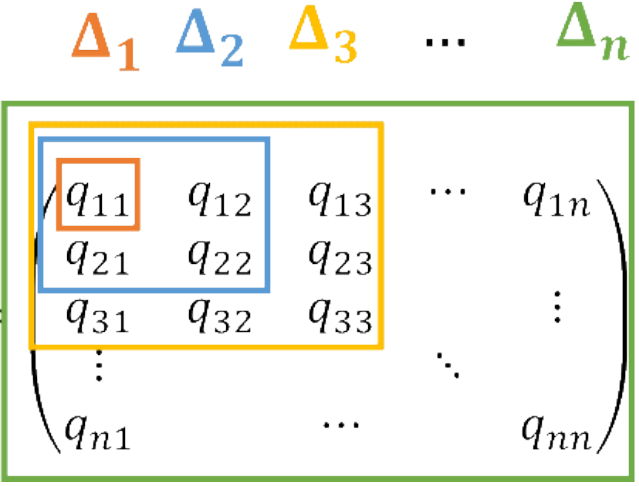
\includegraphics[width=0.3\linewidth]{sylv.png}
% \end{figure}
% \begin{block}{Theorem}
%     A symmetric matrix $A$ is positive definite if and only if all the determinants of its upper-left submatrices are positive.

% \end{block}
% That is, $\Delta_1>0$, $\Delta_2>0$, \dots, $\Delta_n>0$.
% \pause

% \begin{block}{Theorem}

%     A symmetric matrix $A$ is negative definite if and only if the determinants of its odd upper-left submatrices are negative, even submatrices positive. 
% \end{block}
% That is, $\Delta_1<0$, $\Delta_2>0$, $\Delta_3<0$, \dots
% \end{frame}



\end{document}
